% Todo:

\documentclass[12pt]{article}
\usepackage{hyperref}
\usepackage{xeCJK}
\usepackage{fontspec}
%\setCJKmainfont{SimSun}
\setCJKmainfont[BoldFont=SimHei,ItalicFont=KaiTi]{SimSun}
% \setCJKsansfont{SimHei}
% \setCJKmonofont{SimKai}
\setmainfont{Arial}

\usepackage{cite}
\usepackage{graphicx}
\usepackage{float}
\usepackage{amsfonts}
% \usepackage{amsmath}	% for \tag
\usepackage{amssymb}	% for \multimap
% \usepackage{stmaryrd}
\usepackage{color}
%\usepackage[square,numbers]{natbib}
%\nocopyright
%\usepackage{latexsym,amsmath,amssymb,graphicx,hyperref}
%\usepackage{times} % gives you a bit more space if needed
\usepackage{titlesec}		% change color of section headings
\usepackage{verbatim}

\makeatletter
\newsavebox{\@brx}
\newcommand{\llangle}[1][]{\savebox{\@brx}{\(\m@th{#1\langle}\)}%
  \mathopen{\copy\@brx\kern-0.5\wd\@brx\usebox{\@brx}}}
\newcommand{\rrangle}[1][]{\savebox{\@brx}{\(\m@th{#1\rangle}\)}%
  \mathclose{\copy\@brx\kern-0.5\wd\@brx\usebox{\@brx}}}
\makeatother

\titleformat{\section}
{\color{blue}\normalfont\Large\bfseries}
{\color{blue}\thesection}{1em}{}
\titleformat{\subsection}
{\color{blue}\normalfont\large\bfseries}
{\color{blue}\thesubsection}{1em}{}

\renewcommand\abstractname{\textcolor{blue}{Abstract}}

\definecolor{LogicColor}{rgb}{0.4,0.1,0.4}  % Magenta
% \definecolor{LogicColor}{rgb}{0,0,0}	% for black-and-white paper

\newcommand{\concept}[1]{\textbf{\textcolor{blue}{#1}}}

\newcommand{\english}[1]{\rmfamily \textit{``#1''}\rmfamily}
\newcommand{\formula}[1]{\textcolor{LogicColor}{#1}}

\newcommand{\df}{f} %probability density function
\newcommand{\dfo}{f1} %other probability density function
\newcommand{\fv}{x} %fuzzy variable
\newcommand{\tab}{\hspace*{1cm}}
\newcommand{\zand}{\; \tilde{\wedge} \;}
\newcommand{\zor}{\; \tilde{\vee} \;}
\newcommand{\PimpL}{\leftarrowtriangle}
\newcommand{\com}{\multimap}
\newcommand{\comL}{\circ \hspace{-0.4em} - \,}
\newcommand{\mul}{}
\newcommand{\loves}{loves }
\newcommand{\heart}{\, \heartsuit \,}

\newcommand*\sigmoid{\vcenter{\hbox{
\includegraphics{sigmoid.png}}}}
\newcommand*\sadface{
\includegraphics[scale=0.25]{face-sad.png}}

\setlength{\oddsidemargin}{1cm}
\setlength{\evensidemargin}{1cm}
\setlength{\textwidth}{14cm}

\title{\textcolor{blue}{Genifer 4.2 theoretical notes}}
\author{YKY (\textit{甄景贤})}
%\date{27 May 2015}
% \institute{}

\begin{document}

\tab\tab\tab \parbox{10cm}{\textit{I recall with amusement Eckert's reaction to the impending visit. He said that he could tell whether von Neumann was really a genius by his first question. If this was about the logical structure of the machine, he would believe in von Neumann, otherwise not. Of course this was von Neumann's first query.}}
% \vspace{-0.5cm}
\begin{flushright}
\textemdash\, Goldstine \\The Computer from Pascal to von Neumann [1972]
\end{flushright}

\sffamily

{\let\newpage\relax\maketitle}

\maketitle
\setlength{\parindent}{0em}
\setlength{\parskip}{1.5ex plus0.5ex minus1.2ex}

Let me recap a bit, what I've been trying to do....

%首先,我们有一个原子概念的集合 $A = \{ \mbox{男人}, \mbox{女人}, \mbox{爱}, \mbox{恨}, \mbox{足球},... \}$,在抽象代数中这个集通常叫作 alphabet,它的元素叫字母 (letters)。 

In 2013, Tom\'{a}\v{s} Mikolov et al in Google created \textbf{Word2Vec}, that became very influential.  Basically it associates to each (English) word a vector in continuous space (that requires some form of approximation), and this approximation is based on the \textbf{Distributional Hypothesis}, which says, ``words that are used and occur in the same contexts tend to purport similar meanings''.

My purpose is not to explore how to calculate the distributive representation of words (or concepts), but to build upon this representation of primitive concepts, assuming that this task is completed, whether it uses Word2Vec or some other methods.

% 给定一个字 $w$,Word2Vec 计算它最有可能的上下文 $c$,而 $c$ 是用参数 $\theta$ 给出的:
% $$ \arg \max_\theta \prod_{(w,c) \in D} p(c|w; \theta) $$

Our goal is to pass from \textbf{words} to \textbf{sentences}, and then to perform \textbf{deduction} and \textbf{inductive learning} over sentences.

\section{Deduction}

%Define the notion of \textbf{cognitive state}:  In classical logic-based AI the KB stores logical \textbf{facts}, and additionally there is a store of logical \textbf{rules}.  We can regard a set of facts as a \textbf{cognitive state}, and rules act on a cogitive state to change it into another cognitive state.  In other words, a cognitive state is the set of facts currently believed to be true and are under conscious attention (ie, present in working memory).

In classical logic-based AI, a set of logical rules \textbf{acts on} logical facts to give rise to new facts.  We can denote the set of facts as $G$, the \textbf{cognitive state} of the system.  Thus the rules $R$ act on $G$:
\begin{eqnarray}
 R: G \mapsto G \nonumber \\
 R : \mathbf{G} \rightarrow \mathbf{G} \nonumber
\end{eqnarray}

Notation:
\begin{eqnarray}
G &=& \mbox{a single cognitive state} \nonumber \\
\mathbf{G} &=& \mbox{space of all cognitive states} \nonumber \\
R : \mathbf{G} \rightarrow \mathbf{G} &=& \mbox{rules operating on cognitive states} \nonumber
\end{eqnarray}

We can also call R the \textbf{single-step deduction operator}.

The goal of \textbf{inductive learning} is to learn the set of rules $R$.

So far, this is classical AI.

In the new formulation, sentences (or logical statements) are built up from words (or atomic concepts).  Words can be placed in vector space via algorithms such as Word2Vec.  Sentences can constructed from words via tensor products (there are multiple ways to do this, and we will explore this later), and such a sentence representation inherits the vector space structure of words.  The KB\footnote{or more precisely, the facts base, ie the cognitive state $G$} is a collection (set union) of sentences.  All in all, the cognitive state $G$ can be represented in vector space.

So, without change in notation, but now $G \in \mathbf{G}$ is a vector, $\mathbf{G}$ is a vector space, $R$ is an \textit{operator} acting on $\mathbf{G}$:
\begin{eqnarray}
 R: G \mapsto G \nonumber \\
 R : \mathbf{G} \rightarrow \mathbf{G} \nonumber
\end{eqnarray}

\subsection{Continuous relaxation}

Without explicitly saying so, we have already \textit{relaxed} $R$ so that it need not correspond to a single logical deduction step.  Look at this chain of deduction:
$$ G_0 \stackrel{R}{\longrightarrow} G_1 \stackrel{R}{\longrightarrow} ... \stackrel{R}{\longrightarrow} G_\infty $$
where $G_\infty$ is the final cognitive state (we want to train $R$ to give rise to an ideal final state $G^*$).  We do not require $R$ to correspond to the \textit{discrete} steps of logical deduction.  $R$ can be ``fractional'' or even ``infinitesimal'', ie, it changes $G$ by just a small (or infinitesimal) amount.  This might be a good feature to have.

\section{Integrating with reinforcement learning}

Richard Sutton's view is that the \textbf{reinforcement learner (RL)} should be the \textit{top-level} architecture of an AI, which I agree.\footnote{see my introductory \href{http://geniferology.blogspot.hk/2015/05/what-is-reinforcement-learning.html}{blog article} on reinforcement learning}

So the logic sub-system would be a module inside the RL.  Question is how to link the RL with the logic module.  Sutton has also mentioned, that the challenge in reinforcement learning is how to give the RL an efficient \textbf{world model}, and I think that role is to be filled by the logic sub-system.  Without a world model, the RL only has knowledge about state transitions, and the real world has an astronomical number of states.  The logic sub-system \textit{condenses} world knowledge into generalized logic statements.

The RL can be viewed as a black box that inputs $\{ states, actions, rewards \}$ and outputs a $policy$.  In order for RL to control the logic sub-system, we need to view the logic inference engine as a machine with controls.  What are the internal \textbf{states} of this engine?  What are the \textbf{actions} that transform the states?  What are the rewards?

I don't have a solution yet, just a few points:

\subsection{Logic as an external teacher}

\begin{figure}[H]
\centering

\includegraphics[scale=0.25]{boomerang.jpg}
\end{figure}

Say you have a boomerang, you learn to throw the boomerang so that it flies back to you beautifully.  That is the job of the RL, to learn how to act in the real world.  The logic sub-system can also be viewed as an object in the real world, which we could \textit{manipulate}.  But something is tricky here: the inference engine \textit{itself} derives logical conclusions to advice the RL on decisions and actions.

Think carefully, there is no ``bad recursion'' here.  The inference engine can be regarded as a teacher.  It suggests to the RL some actions.  The RL can accept or deny to perform those actions.  If it does accept, the RL observes how good is the outcome.  Then it can \textit{adjust} or \textit{fine tune} the teacher accordingly.  In the entire process above, the teacher is an \textit{external} entity manipulated by the RL.

\subsection{How to invoke the inference engine?}

On the highest level, the inference engine can only perform 2 actions:  deduction and inductive learning.  We need to \textit{refine} these actions so the RL can ``micro-control'' the inference engine.

The rewards should be passed from the RL itself, as we have no other way to know what is desirable for the system.

Think of a chain of logical inference:
$$ \Gamma \vdash \Delta \vdash \Lambda \; ... ... \vdash \mbox{``I decide to pee''} $$
and this should result in an act of urination.  This means that we should recognize and allow certain logic statements to trigger real-world actions (such real-world actions should not be confused with the inference engine's internal actions, the latter I call \textbf{control actions}).

We can put data into the KB to cause the inference engine to perform specific reasoning tasks.  For example, ``I am in the middle of a busy street, I feel like urinating, should I pee?''

In my model, the cognitive state vector can also store \textit{internal} or \textit{intermediate} variables, similar to the registers of a Turing machine \footnote{That is the similarity between my model and Neural Turing Machines. The Turing machine's basic operations are \textit{read}, \textit{write} and \textit{move tape}, which are very primitive.  Whereas my model can perform logical operations which are much more advanced.}.  

So the RL can alter $G$ to control the inference engine's performance (these are the control actions from the RL's perspective).  The state of the inference engine is $G$, and the rewards are observed from how well the logic engine performs as a teacher.

\section{Tensor product representations}

\begin{itemize}
\item The most basic is the relation $a \, R \, b$ with 3 elements
\item Smolensky's method, which can represent any recursive tree structure
\item In a fairly new research direction, people realize that linguistic structure is identical to abstract algebraic structure, so attention is shifted to studying abstract categories.  For example this book:
\begin{figure}[H]
\centering
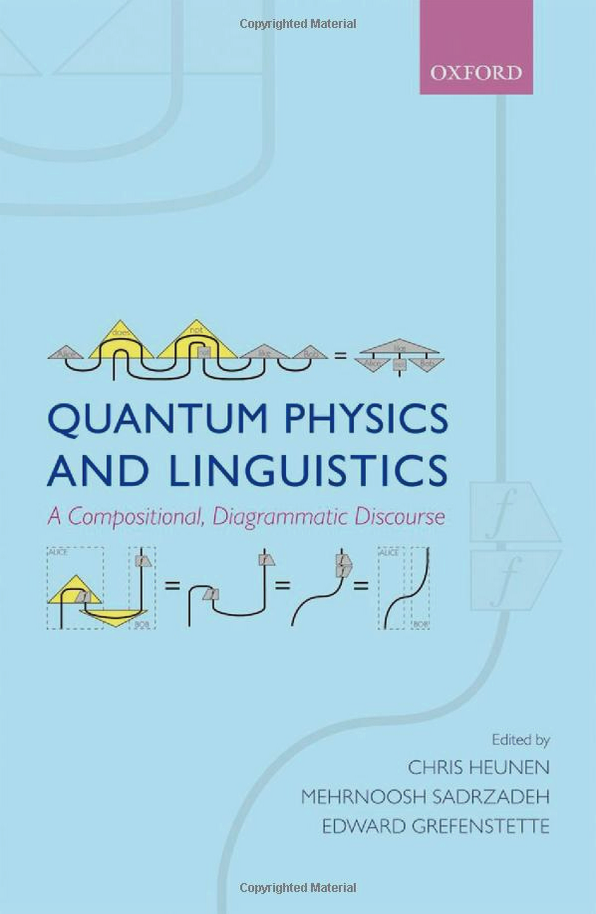
\includegraphics[scale=0.3]{quantum-physics-and-linguistics-book-cover.png}
\end{figure}
\end{itemize}

The most general categories are \textbf{monoidal categories}, also called \textbf{tensor categories}.  The tensor product of vector spaces is an example in this category.  Essentially we are using tensor products to represent sentences;  Category theory provides a more general and abstract framework.

\subsection{Neural Tensor Network}

Andrew Ng is from Hong Kong, he taught a famous machine learning course in Coursera.  Recently he left Stanford to join Baidu (the Chinese search engine).

Socher, Chen, Manning, and Ng proposed the NTN model in 2013 \cite{Socher2013}:
$$ \top(a\, R\, b) = u^T \; \sigmoid \, (a^T \, U \, b + W {{a}\choose{b}} + c ) $$
$\top(a\, R\, b)$ is the \textbf{strength} of the relation $a\, R\, b$.\\
$U$ is a tensor, it takes two vectors $a, b$ and gives a third vector $a^T \, U \, b$ (this obeys the bi-linear property of tensors).\\
$W$ is a matrix, $W {{a}\choose{b}}$ is a layer of traditional neural network, $\sigmoid$ is a non-linear threshold function.\\
$u^T$ is a single neuron, it's purpose is to add up the different components, giving a number.

\subsection{Paul Smolensky}

Paul Smolensky's book is \textit{The Harmonic Mind} (2006)\cite{Smolensky2006}.  Volume 1 is AI theory, Volume 2 is linguistic theory.
\begin{figure}[H]
\centering
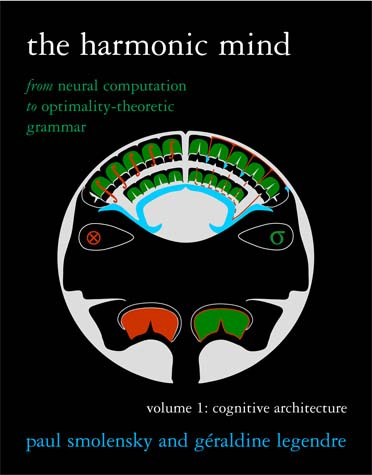
\includegraphics[scale=0.5]{the-harmonic-mind-cover.jpg}
\end{figure}

He suggests to use tensors to represent relations;  Generally speaking:
\begin{eqnarray}
father(john, pete) & \Leftrightarrow & father \otimes john \otimes pete \nonumber \\
Var_1 : val_1, Var_2 : val_2 & \Leftrightarrow & Var_1 \otimes val_1 + Var_2 \otimes val_2 \nonumber 
\end{eqnarray}
The second line means: $variable_1$ takes value $value_1$,$variable_2$ takes value $value_2$.

He also introduced the notions of ``roles'' and ``fillers'': $variable_i$ is a role, $value_i$ is a filler.  Using this method to handle variable binding, the advantage is that it can avoid the $ A \cdot B = B \cdot A $ problem.

For example, in natural language we could have a sentence structure like this:
$$ s = \quad \raisebox{-.5\height}{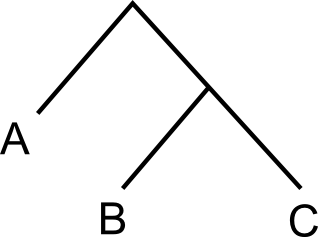
\includegraphics[scale=0.75]{Smolensky-tree.png}} $$

$r_0$ and $r_1$ are respectively the tree's left and right children's roles.  Expressed as a tensor product:
\begin{eqnarray}
s &=& A \otimes r_0 + q \otimes r_1 \nonumber \\
q &=& B \otimes r_0 + C \otimes r_1 \nonumber \\
\therefore \; s &=& A \otimes r_0 + B \otimes r_0 \otimes r_1 + C \otimes r_1 \otimes r_1 \nonumber
\end{eqnarray}

The good thing about tensor products is that, $r_0$ and $r_0 \otimes r_1$ are different elements, they would not "clash".  A drawback is that as the length of the tensor product grows, its dimension also grows very fast.

The following table summarizes Smolensky's approach:
\begin{center}
\begin{tabular}{|c|c|c|}
\hline
                    & Example & Vector representation \\
\hline
Set element         & $\{ c_1, c_2 \}$ & $ c_1 + c_2 $ \\ 
\hline
Filler-role binding & $ AB = \{ A \backslash r_1, B \backslash r_2\} $ & $ A \otimes r_0 + B \otimes r_1 $\\
\hline
Recursive structure & \raisebox{-.5\height}{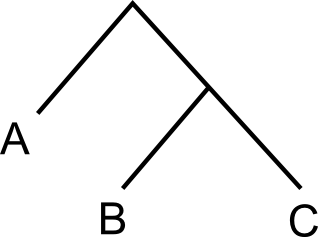
\includegraphics[scale=0.5]{Smolensky-tree.png}} & $A \otimes r_0 + [BC] \otimes r_1$ \\
\hline
\end{tabular}
\end{center}

% 和我的 naive 办法相比,有什么分别?  

As I have explained on my blog \footnote{\href{http://geniferology.blogspot.hk/2015/03/what-are-tensors.html}{blog post}} before, tensors are the universal form of all bi-linear forms.  If we have 2 vector spaces $U$ and $V$,
\begin{eqnarray}
T: & U \otimes V \rightarrow W \nonumber \\
t: & u \otimes v \mapsto w \nonumber 
\end{eqnarray}
and 2 sets of vectors in $U, V$ that are linearly independent, $\{u_1, ..., u_m \}$ and $\{ v_1, ..., v_n \}$, then their product $\{ u_i \otimes v_i \}$ in $W$ would still be linearly-independent.  This is a \textit{defining property} of tensor products, in other words:
$$ \mbox{linear independent set} \otimes \mbox{linear independent set} \mapsto \mbox{linear independent set} $$
and this is precisely what we need, because under the ``scalar = logic truth value'' interpretation, this is precisely the condition where propositions would not ``clash''.

Antony Browne \& Ron Sun's earlier paper ``Connectionist Inference Models'' (2001) \cite{Browne2001} talks more about various neural-symbolic integration schemes.

\subsection{Coecke-Sadrzadeh-Clark}

This representation is proposed by Coecke, Sadrzadeh, Clark in 2010 \cite{Coecke2010}.

Firstly it is based on \textbf{categorial grammar}, which is a grammar with ``left'' and ``right'' multiplications.  For example, in the sentence \english{John likes Mary}, the type of \english{likes} is:
$$ likes := (S\backslash NP)/NP $$
That means when the word \english{likes} is multiplied by a noun phrase on the left, and another noun phrase on the right, we obtain a sentence S.  This kind of grammar is pioneered by Lambek in 1958.

Translating to tensor products, \english{likes} is represented as a vector:
$$ \overrightarrow{likes} \in N \otimes S \otimes N $$
which makes sense, because this tensor product space contains as elements the multi-linear functions:
$$ f : N \times N \rightarrow S. $$

%\section*{Appendix: XXXX}

%\section*{Acknowledgments}

\bibliographystyle{plain} % or number or aaai ...
\bibliography{AGI-book}

%\onecolumn

% Bigger figures

\end{document}
